\documentclass{article}
\usepackage[utf8]{inputenc}

% Essential packages for article format
\usepackage{amsmath, amssymb, amsfonts}
\usepackage{bm}
\usepackage{graphicx}
\usepackage{xcolor}
\usepackage{tcolorbox}
\usepackage[bookmarks=false]{hyperref}
\usepackage{url}
\usepackage{booktabs}
\usepackage{array}
\usepackage{multirow}
\usepackage{enumitem}
\usepackage{tikz}
\usetikzlibrary{arrows.meta, positioning, shapes.geometric}

% Additional packages for a nice tutorial format
\usepackage[margin=1in]{geometry}
\usepackage{fancyhdr}
\usepackage{titlesec}

% Header and footer setup
\pagestyle{fancy}
\fancyhf{}
\rhead{Tutorial 0: Mathematical Prerequisites}
\lhead{ES335 - Machine Learning}
\rfoot{Page \thepage}

% Title formatting
\titleformat{\section}{\Large\bfseries\color{blue!75!black}}{\thesection}{1em}{}
\titleformat{\subsection}{\large\bfseries\color{blue!60!black}}{\thesubsection}{1em}{}

% Load conventions after math packages
\usepackage{../../shared/styles/conventions}

% Define counters for examples and exercises
\newcounter{example}
\setcounter{example}{0}
\newcounter{exercise}
\setcounter{exercise}{0}

\title{\textbf{Tutorial 0: Mathematical Prerequisites for Machine Learning} \\ \textit{Scalars, Vectors, Matrices, Probability, and Statistics}}
\author{ES335 - Machine Learning \\ IIT Gandhinagar}
\date{\today}

\begin{document}

\maketitle

\begin{abstract}
This tutorial covers essential mathematical concepts that are fundamental to understanding machine learning algorithms. We start with basic building blocks (scalars, vectors, matrices) and progress to more advanced topics (norms, rank, probability, statistics). Each concept is explained with intuitive examples from real-world scenarios, followed by both simple and challenging exercises to test your understanding.
\end{abstract}

\tableofcontents
\newpage

\section{Introduction: Why These Math Concepts Matter}

Imagine you're developing a recommendation system for Netflix. You have:
\begin{itemize}
    \item \textbf{Scalars}: A single user's rating (4.2 stars) for a movie
    \item \textbf{Vectors}: All ratings by one user [4.2, 3.1, 5.0, 2.8, ...]
    \item \textbf{Matrices}: Ratings by all users for all movies (millions × millions grid)
    \item \textbf{Norms}: How ``similar'' are two users' preferences?
    \item \textbf{Probability}: What's the chance this user will like a sci-fi movie?
    \item \textbf{Statistics}: What's the average rating for action movies?
\end{itemize}

Understanding these concepts deeply will help you build better ML models and debug them when things go wrong.

\section{Scalars: The Building Blocks}

\subsection{What Are Scalars?}

A \textbf{scalar} is just a single number. In machine learning contexts:
\begin{itemize}
    \item Learning rate: $\alpha = 0.001$
    \item Temperature: $T = 23.5^\circ\text{C}$
    \item Accuracy: $acc = 0.94$
    \item Loss value: $L = 2.317$
\end{itemize}

\begin{tcolorbox}[colback=green!5!white,colframe=green!75!black,title=Example \stepcounter{example}\#\theexample: House Price Prediction]
You're predicting house prices. Here are some scalars in your model:
\begin{itemize}
    \item House size: 1,850 square feet
    \item Number of bedrooms: 3
    \item Predicted price: \$425,000
    \item Model's confidence: 0.87
\end{itemize}
Each of these is a scalar because it's a single number representing one quantity.
\end{tcolorbox}

\subsection{Scalar Operations}

When working with scalars, you can perform basic arithmetic:
\begin{align}
a + b &= 5 + 3 = 8 \\
a \times b &= 5 \times 3 = 15 \\
a^b &= 5^3 = 125 \\
\sqrt{a} &= \sqrt{25} = 5
\end{align}

\begin{center}
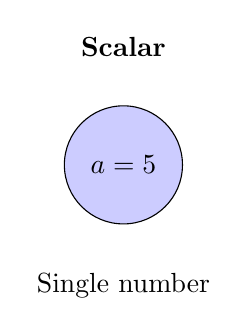
\begin{tikzpicture}
    \node[circle, draw, fill=blue!20, minimum size=1.5cm] (scalar) at (0,0) {$a = 5$};
    \node[above=0.5cm of scalar] {\textbf{Scalar}};
    \node[below=0.5cm of scalar] {Single number};
\end{tikzpicture}
\end{center}

\section{Vectors: Lists of Related Numbers}

\subsection{Understanding Vectors Intuitively}

A \textbf{vector} is an ordered list of numbers. Think of it as:
\begin{itemize}
    \item Your location in GPS coordinates: [latitude, longitude]
    \item Stock prices: [AAPL: \$150, GOOGL: \$2800, MSFT: \$300]
    \item Image pixels: [red\_value, green\_value, blue\_value] for each pixel
\end{itemize}

\begin{tcolorbox}[colback=blue!5!white,colframe=blue!75!black,title=Example \stepcounter{example}\#\theexample: Student Performance Vector]
A student's performance across different subjects:
$$\vx = \begin{bmatrix} 85 \\ 92 \\ 78 \\ 96 \\ 88 \end{bmatrix} \leftarrow \begin{matrix} \text{Math} \\ \text{Physics} \\ \text{Chemistry} \\ \text{Computer Science} \\ \text{English} \end{matrix}$$

This vector $\vx \in \Real^5$ captures the student's complete academic profile in one mathematical object.
\end{tcolorbox}

\subsection{Vector Visualization}

\begin{center}
\begin{tikzpicture}[scale=1.5]
    % Draw coordinate system
    \draw[->] (-0.5,0) -- (4,0) node[right] {$x_1$};
    \draw[->] (0,-0.5) -- (0,3) node[above] {$x_2$};
    
    % Draw vector
    \draw[->, thick, red] (0,0) -- (3,2) node[midway, above left] {$\vx = \begin{bmatrix} 3 \\ 2 \end{bmatrix}$};
    
    % Draw components
    \draw[dashed, blue] (3,0) -- (3,2);
    \draw[dashed, blue] (0,2) -- (3,2);
    
    \node[below] at (1.5,0) {$x_1 = 3$};
    \node[left] at (0,1) {$x_2 = 2$};
    
    \node[above right] at (3,2) {$(3,2)$};
\end{tikzpicture}
\end{center}

\subsection{Common Vector Operations}

\textbf{1. Vector Addition (Element-wise)}
$$\vx + \vy = \begin{bmatrix} 2 \\ 3 \end{bmatrix} + \begin{bmatrix} 1 \\ 4 \end{bmatrix} = \begin{bmatrix} 3 \\ 7 \end{bmatrix}$$

\textbf{2. Scalar Multiplication}
$$3 \cdot \vx = 3 \cdot \begin{bmatrix} 2 \\ 3 \end{bmatrix} = \begin{bmatrix} 6 \\ 9 \end{bmatrix}$$

\textbf{3. Dot Product (Inner Product)}
$$\vx \cdot \vy = \vx^T \vy = \sum_{i=1}^d x_i y_i$$

\begin{tcolorbox}[colback=orange!5!white,colframe=orange!75!black,title=Example \stepcounter{example}\#\theexample: Movie Recommendation Dot Product]
User A's movie ratings: $\vx = [5, 3, 4, 2, 5]$ (Action, Comedy, Drama, Horror, Sci-Fi)\\
User B's movie ratings: $\vy = [4, 4, 5, 1, 4]$

Similarity (dot product): $\vx \cdot \vy = 5 \times 4 + 3 \times 4 + 4 \times 5 + 2 \times 1 + 5 \times 4 = 74$

Higher dot product suggests similar tastes!
\end{tcolorbox}

\section{Matrices: Tables of Numbers}

\subsection{Matrix Intuition}

A \textbf{matrix} is a rectangular array of numbers. Think of it as:
\begin{itemize}
    \item Spreadsheet with rows and columns
    \item Collection of vectors stacked together
    \item Transformation that changes vectors
\end{itemize}

\begin{center}
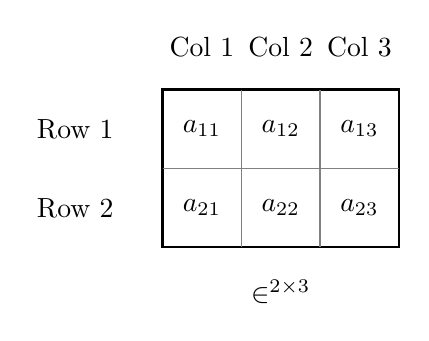
\begin{tikzpicture}
    % Draw matrix visualization
    \draw[thick] (0,0) rectangle (3,2);
    \draw[gray] (1,0) -- (1,2);
    \draw[gray] (2,0) -- (2,2);
    \draw[gray] (0,1) -- (3,1);
    
    \node at (0.5,1.5) {$a_{11}$};
    \node at (1.5,1.5) {$a_{12}$};
    \node at (2.5,1.5) {$a_{13}$};
    \node at (0.5,0.5) {$a_{21}$};
    \node at (1.5,0.5) {$a_{22}$};
    \node at (2.5,0.5) {$a_{23}$};
    
    \node[below] at (1.5,-0.3) {$\mA \in \Real^{2 \times 3}$};
    \node[left] at (-0.5,1.5) {Row 1};
    \node[left] at (-0.5,0.5) {Row 2};
    \node[above] at (0.5,2.3) {Col 1};
    \node[above] at (1.5,2.3) {Col 2};
    \node[above] at (2.5,2.3) {Col 3};
\end{tikzpicture}
\end{center}

\begin{tcolorbox}[colback=purple!5!white,colframe=purple!75!black,title=Example \stepcounter{example}\#\theexample: Student Grades Matrix]
Grades for 3 students across 4 subjects:
$$\mX = \begin{bmatrix} 
85 & 92 & 78 & 96 \\
90 & 88 & 85 & 94 \\
82 & 95 & 80 & 91
\end{bmatrix} \leftarrow \begin{matrix} \text{Alice} \\ \text{Bob} \\ \text{Carol} \end{matrix}$$
$$\uparrow \quad \uparrow \quad \uparrow \quad \uparrow$$
$$\text{Math} \quad \text{Physics} \quad \text{Chem} \quad \text{CS}$$

Each row is a student's performance vector. Each column is all students' performance in one subject.
\end{tcolorbox}

\subsection{Matrix Operations}

\textbf{Matrix Multiplication} (Most Important!)
$$\mA \mB = \mC \text{ where } c_{ij} = \sum_{k=1}^p a_{ik} b_{kj}$$

\textbf{Key Rule}: $(m \times n) \times (n \times p) = (m \times p)$

\begin{center}
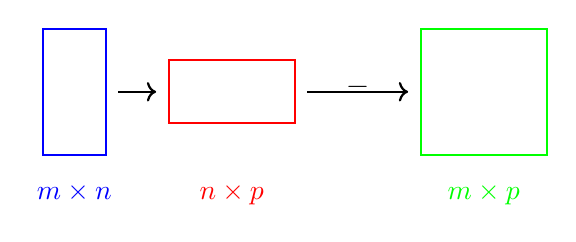
\begin{tikzpicture}[scale=0.8]
    % Draw matrices
    \draw[thick, blue] (0,0) rectangle (1,2);
    \node at (0.5,1) {\color{blue}$\mA$};
    \node[below, blue] at (0.5,-0.3) {$m \times n$};
    
    \draw[thick, red] (2,0.5) rectangle (4,1.5);
    \node at (3,1) {\color{red}$\mB$};
    \node[below, red] at (3,-0.3) {$n \times p$};
    
    \node at (5,1) {$=$};
    
    \draw[thick, green] (6,0) rectangle (8,2);
    \node at (7,1) {\color{green}$\mC$};
    \node[below, green] at (7,-0.3) {$m \times p$};
    
    \draw[->, thick] (1.2,1) -- (1.8,1);
    \draw[->, thick] (4.2,1) -- (5.8,1);
\end{tikzpicture}
\end{center}

\section{Vector and Matrix Norms}

\subsection{What Are Norms?}

A \textbf{norm} measures the ``size'' or ``length'' of a vector/matrix. Think of it as:
\begin{itemize}
    \item Distance from origin to a point
    \item Magnitude of a force vector
    \item ``How big'' is this mathematical object?
\end{itemize}

\subsection{Common Vector Norms}

\textbf{1. L1 Norm (Manhattan Distance)}
$$\normone{\vx} = \sum_{i=1}^n |x_i|$$

Like walking in Manhattan - you can only go up/down, left/right.

\textbf{2. L2 Norm (Euclidean Distance)}
$$\normtwo{\vx} = \sqrt{\sum_{i=1}^n x_i^2}$$

Straight-line distance ``as the crow flies.''

\textbf{3. L$\infty$ Norm (Maximum Norm)}
$$\norminf{\vx} = \max_i |x_i|$$

Just the largest component.

\begin{center}
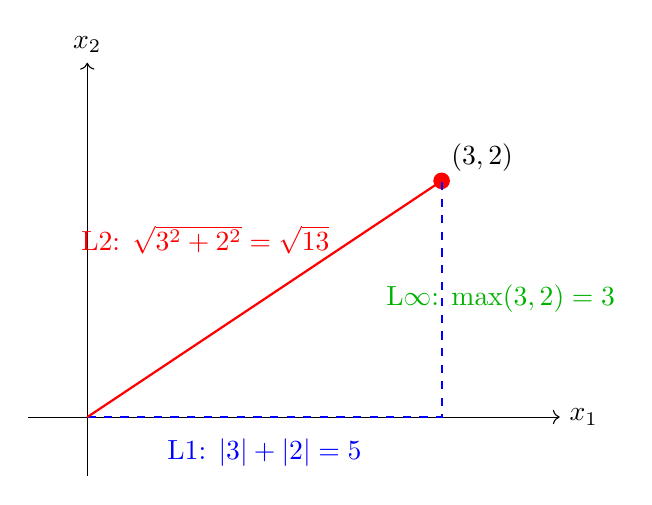
\begin{tikzpicture}[scale=1.5]
    % Coordinate system
    \draw[->] (-0.5,0) -- (4,0) node[right] {$x_1$};
    \draw[->] (0,-0.5) -- (0,3) node[above] {$x_2$};
    
    % Point
    \fill[red] (3,2) circle (2pt);
    \node[above right] at (3,2) {$(3,2)$};
    
    % L1 path
    \draw[thick, blue, dashed] (0,0) -- (3,0) -- (3,2);
    \node[blue] at (1.5,-0.3) {L1: $|3| + |2| = 5$};
    
    % L2 path
    \draw[thick, red] (0,0) -- (3,2);
    \node[red] at (1,1.5) {L2: $\sqrt{3^2 + 2^2} = \sqrt{13}$};
    
    % L∞
    \node[green!70!black] at (3.5,1) {L$\infty$: $\max(3,2) = 3$};
\end{tikzpicture}
\end{center}

\begin{tcolorbox}[colback=cyan!5!white,colframe=cyan!75!black,title=Example \stepcounter{example}\#\theexample: Error Vector Norms]
Your model's prediction errors on 4 test samples: $\text{errors} = [2, -1, 3, -4]$

\begin{itemize}
    \item L1 norm: $\normone{errors} = 2 + 1 + 3 + 4 = 10$ (total absolute error)
    \item L2 norm: $\normtwo{errors} = \sqrt{4 + 1 + 9 + 16} = \sqrt{30}$ (root mean square error)
    \item L$\infty$ norm: $\norminf{errors} = 4$ (worst single error)
\end{itemize}

Different norms emphasize different aspects of your model's performance!
\end{tcolorbox}

\section{Matrix Rank and Linear Independence}

\subsection{Understanding Rank Intuitively}

The \textbf{rank} of a matrix tells you:
\begin{itemize}
    \item How many ``truly different'' rows/columns it has
    \item The dimension of the space it spans
    \item Whether the matrix is invertible
\end{itemize}

\begin{tcolorbox}[colback=yellow!5!white,colframe=yellow!75!black,title=Example \stepcounter{example}\#\theexample: Student Survey Matrix]
Survey responses from 3 students on 3 questions (1-5 scale):
$$\mA = \begin{bmatrix} 
5 & 4 & 3 \\
4 & 3 & 2 \\
3 & 2 & 1
\end{bmatrix}$$

Notice: Row 2 = Row 1 - 1, Row 3 = Row 1 - 2

This matrix has rank 1 because all rows are multiples of the first row!
\end{tcolorbox}

\subsection{Key Properties}
\begin{itemize}
    \item For $\mA \in \Real^{m \times n}$: $\text{rank}(\mA) \leq \min(m,n)$
    \item \textbf{Full rank}: $\text{rank}(\mA) = \min(m,n)$
    \item Square matrix is \textbf{invertible} iff it has full rank
    \item Low rank often means redundant information
\end{itemize}

\section{Probability Fundamentals}

\subsection{Why Probability in ML?}

Machine learning is fundamentally about dealing with uncertainty:
\begin{itemize}
    \item Will this email be spam? (Classification uncertainty)
    \item What's the range of possible house prices? (Regression uncertainty)  
    \item How confident is my model? (Model uncertainty)
\end{itemize}

\subsection{Basic Probability Concepts}

\textbf{Sample Space} ($\Omega$): All possible outcomes
\textbf{Event} ($A$): A subset of the sample space
\textbf{Probability} ($P(A)$): How likely an event is

\textbf{Properties}:
\begin{align}
0 \leq P(A) &\leq 1 \\
P(\Omega) &= 1 \\
P(A \cup B) &= P(A) + P(B) - P(A \cap B)
\end{align}

\begin{tcolorbox}[colback=red!5!white,colframe=red!75!black,title=Example \stepcounter{example}\#\theexample: Email Classification]
Your spam filter processes 1000 emails:
\begin{itemize}
    \item 200 are spam
    \item 800 are not spam
    \item Of spam emails, 180 contain word ``free''
    \item Of non-spam emails, 50 contain word ``free''
\end{itemize}

Probabilities:
\begin{align}
P(\text{spam}) &= \frac{200}{1000} = 0.2 \\
P(\text{"free"}) &= \frac{180 + 50}{1000} = 0.23 \\
P(\text{"free"}|\text{spam}) &= \frac{180}{200} = 0.9
\end{align}
\end{tcolorbox}

\subsection{Conditional Probability and Bayes' Theorem}

\textbf{Conditional Probability}: $P(A|B) = \frac{P(A \cap B)}{P(B)}$

\textbf{Bayes' Theorem}: $P(A|B) = \frac{P(B|A) P(A)}{P(B)}$

This is the foundation of Naive Bayes classifiers!

\begin{center}
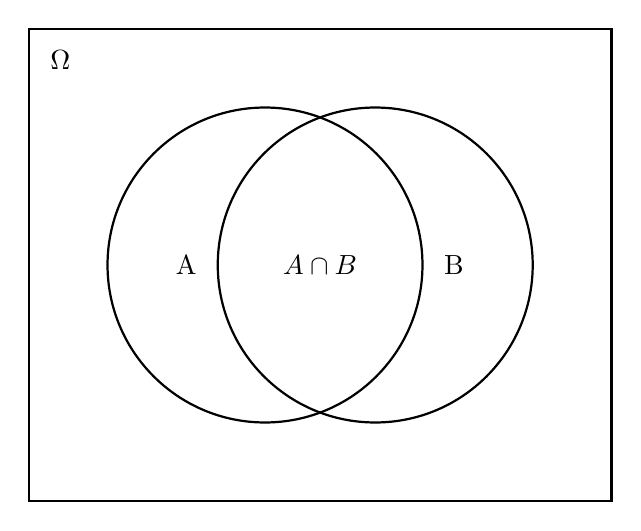
\begin{tikzpicture}[scale=2]
    % Draw Venn diagram
    \draw[thick] (0,0) circle (1);
    \draw[thick] (0.7,0) circle (1);
    
    \node at (-0.5,0) {A};
    \node at (1.2,0) {B};
    \node at (0.35,0) {$A \cap B$};
    
    \draw[thick] (-1.5,-1.5) rectangle (2.2,1.5);
    \node at (-1.3,1.3) {$\Omega$};
\end{tikzpicture}
\end{center}

\section{Statistics: Making Sense of Data}

\subsection{Descriptive Statistics}

\textbf{Central Tendency}:
\begin{align}
\text{Mean: } \mu &= \frac{1}{n}\sum_{i=1}^n x_i \\
\text{Median: } &\text{middle value when sorted} \\
\text{Mode: } &\text{most frequent value}
\end{align}

\textbf{Variability}:
\begin{align}
\text{Variance: } \sigma^2 &= \frac{1}{n}\sum_{i=1}^n (x_i - \mu)^2 \\
\text{Standard Deviation: } \sigma &= \sqrt{\sigma^2}
\end{align}

\begin{tcolorbox}[colback=teal!5!white,colframe=teal!75!black,title=Example \stepcounter{example}\#\theexample: Model Performance Analysis]
Your model's accuracy across 10 different test sets:
$$\text{accuracies} = [0.85, 0.87, 0.83, 0.89, 0.86, 0.88, 0.84, 0.90, 0.85, 0.87]$$

Statistics:
\begin{itemize}
    \item Mean: $\mu = 0.864$ (average performance)
    \item Standard deviation: $\sigma = 0.022$ (consistency)
    \item Range: $[0.83, 0.90]$ (best/worst case)
\end{itemize}

Low standard deviation means your model is consistent!
\end{tcolorbox}

\subsection{Important Distributions}

\textbf{1. Normal Distribution} $\mathcal{N}(\mu, \sigma^2)$
- Bell-shaped, symmetric
- Many real phenomena follow this
- Central Limit Theorem

\textbf{2. Bernoulli Distribution}
- Single coin flip: success/failure
- Parameter: $p$ (probability of success)

\textbf{3. Binomial Distribution}
- Multiple coin flips
- Parameters: $n$ (trials), $p$ (success probability)

\begin{center}
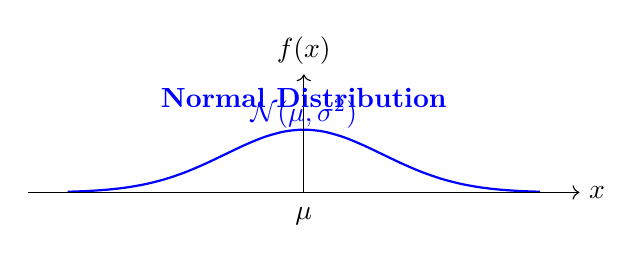
\begin{tikzpicture}[scale=1]
    % Draw normal distribution curve
    \draw[domain=-3:3,smooth,variable=\x,thick,blue] plot ({\x},{2*exp(-\x*\x/2)/sqrt(2*pi)});
    \draw[->] (-3.5,0) -- (3.5,0) node[right] {$x$};
    \draw[->] (0,0) -- (0,1.5) node[above] {$f(x)$};
    
    \node at (0,-0.3) {$\mu$};
    \draw[dashed] (0,0) -- (0,0.8);
    
    \node[blue] at (0,1.2) {\textbf{Normal Distribution}};
    \node[blue] at (0,1.0) {$\mathcal{N}(\mu, \sigma^2)$};
\end{tikzpicture}
\end{center}

\section{Putting It All Together: A Complete Example}

\begin{tcolorbox}[colback=gray!5!white,colframe=gray!75!black,title=Example \stepcounter{example}\#\theexample: Student Performance Analysis System]

You're building a system to predict student performance. Here's how all concepts connect:

\textbf{Data Representation}:
- Student feature vector: $\vx = [study\_hours, attendance, prev\_gpa, sleep\_hours]^T$
- Dataset matrix: $\mX \in \Real^{1000 \times 4}$ (1000 students, 4 features)
- Target vector: $\vy \in \Real^{1000}$ (final exam scores)

\textbf{Mathematical Operations}:
- Normalize features: $\vx_{norm} = \frac{\vx - \mu}{\sigma}$ (statistics)
- Compute similarities: $\text{sim}(\vx_i, \vx_j) = \frac{\vx_i \cdot \vx_j}{\normtwo{\vx_i} \normtwo{\vx_j}}$ (dot product, norms)
- Linear model: $\hat{y} = \vw^T \vx + b$ (matrix-vector multiplication)

\textbf{Analysis}:
- Check if $\mX$ has full rank (are features independent?)
- Use probability to handle uncertainty in predictions
- Apply statistics to evaluate model performance

This single example uses scalars, vectors, matrices, norms, probability, and statistics!
\end{tcolorbox}

\section{Practice Problems}

\subsection{Warm-up Problems}

\begin{tcolorbox}[colback=gray!5!white,colframe=gray!75!black,title=Problem \stepcounter{exercise}\#\theexercise: Basic Vector Operations]
Given vectors $\vx = [3, -2, 1]^T$ and $\vy = [1, 4, -2]^T$:

\textbf{a)} Calculate $\vx + \vy$\\
\textbf{b)} Calculate $\vx \cdot \vy$\\
\textbf{c)} Calculate $\normone{\vx}$, $\normtwo{\vx}$, and $\norminf{\vx}$\\
\textbf{d)} What is the angle between $\vx$ and $\vy$? (Hint: $\cos \theta = \frac{\vx \cdot \vy}{\normtwo{\vx} \normtwo{\vy}}$)

\textbf{Solutions}:
a) $\vx + \vy = [4, 2, -1]^T$
b) $\vx \cdot \vy = 3(1) + (-2)(4) + 1(-2) = -7$
c) $\normone{\vx} = 6$, $\normtwo{\vx} = \sqrt{14}$, $\norminf{\vx} = 3$
d) $\cos \theta = \frac{-7}{\sqrt{14}\sqrt{21}} = \frac{-7}{\sqrt{294}} \approx -0.408$, so $\theta \approx 114^\circ$
\end{tcolorbox}

\begin{tcolorbox}[colback=gray!5!white,colframe=gray!75!black,title=Problem \stepcounter{exercise}\#\theexercise: Matrix Multiplication Dimensions]
For each pair of matrices, determine if multiplication $\mA\mB$ is possible. If yes, give the dimensions of the result:

\textbf{a)} $\mA \in \Real^{3 \times 4}$, $\mB \in \Real^{4 \times 2}$\\
\textbf{b)} $\mA \in \Real^{5 \times 3}$, $\mB \in \Real^{2 \times 7}$\\
\textbf{c)} $\mA \in \Real^{100 \times 50}$, $\mB \in \Real^{50 \times 1}$\\
\textbf{d)} If $\mA\mB = \mC$ where $\mC \in \Real^{6 \times 8}$ and $\mA \in \Real^{6 \times ?}$, what must be the dimensions of $\mB$?

\textbf{Solutions}:
a) Yes, result is $3 \times 2$
b) No, inner dimensions don't match (3 $\neq$ 2)
c) Yes, result is $100 \times 1$ (column vector)
d) $\mA$ must be $6 \times k$ and $\mB$ must be $k \times 8$ for some $k$
\end{tcolorbox}

\subsection{Intermediate Problems}

\begin{tcolorbox}[colback=gray!5!white,colframe=gray!75!black,title=Problem \stepcounter{exercise}\#\theexercise: Rank and Linear Independence]
Consider the matrix:
$$\mA = \begin{bmatrix} 
1 & 2 & 3 \\
2 & 4 & 6 \\
1 & 3 & 5
\end{bmatrix}$$

\textbf{a)} What is the rank of $\mA$?\\
\textbf{b)} Are the columns linearly independent?\\
\textbf{c)} Is $\mA$ invertible?\\
\textbf{d)} Can the system $\mA\vx = \mathbf{b}$ have a unique solution for some vector $\mathbf{b}$?

\textbf{Solutions}:
a) Rank is 2 (row 2 = 2 × row 1, but row 3 is independent)
b) No, because rank < 3
c) No, because it's not full rank
d) No, because the matrix is not invertible
\end{tcolorbox}

\begin{tcolorbox}[colback=gray!5!white,colframe=gray!75!black,title=Problem \stepcounter{exercise}\#\theexercise: Probability and Bayes]
A diagnostic test for a disease has:
\begin{itemize}
    \item 95\% sensitivity (correctly identifies 95\% of sick people)
    \item 90\% specificity (correctly identifies 90\% of healthy people)
    \item Disease prevalence in population: 2\%
\end{itemize}

\textbf{a)} If someone tests positive, what's the probability they actually have the disease?\\
\textbf{b)} If someone tests negative, what's the probability they're actually healthy?\\
\textbf{c)} Why might this test not be very useful for screening?

\textbf{Solutions}:
a) Using Bayes: $P(\text{disease}|\text{+}) = \frac{0.95 \times 0.02}{0.95 \times 0.02 + 0.10 \times 0.98} \approx 0.162$ (only 16.2\%!)
b) $P(\text{healthy}|\text{-}) = \frac{0.90 \times 0.98}{0.90 \times 0.98 + 0.05 \times 0.02} \approx 0.999$ (99.9\%)
c) Low prevalence leads to many false positives, making positive tests unreliable
\end{tcolorbox}

\subsection{Challenging Problems}

\begin{tcolorbox}[colback=gray!5!white,colframe=gray!75!black,title=Problem \stepcounter{exercise}\#\theexercise: Norm Relationships]
For any vector $\vx \in \Real^n$, prove or find counterexamples for:

\textbf{a)} $\norminf{\vx} \leq \normtwo{\vx} \leq \normone{\vx}$\\
\textbf{b)} $\normtwo{\vx} \leq \sqrt{n} \norminf{\vx}$\\
\textbf{c)} $\normone{\vx} \leq n \norminf{\vx}$\\
\textbf{d)} When do we have equality in part (b)?

\textbf{Solutions}:
a) False! Counter: $\vx = [1, 1]^T$ gives $1 \leq \sqrt{2} \leq 2$ $\checkmark$, but $\vx = [1, 0]^T$ gives $1 = 1 > 0$ $\times$
Correct: $\norminf{\vx} \leq \normtwo{\vx} \leq \normone{\vx}$
b) True: $\normtwo{\vx}^2 = \sum x_i^2 \leq n \max_i |x_i|^2 = n \norminf{\vx}^2$
c) True: $\normone{\vx} = \sum |x_i| \leq n \max_i |x_i| = n \norminf{\vx}$
d) When all components have equal magnitude: $|x_1| = |x_2| = \ldots = |x_n|$
\end{tcolorbox}

\begin{tcolorbox}[colback=gray!5!white,colframe=gray!75!black,title=Problem \stepcounter{exercise}\#\theexercise: Covariance Matrix Analysis]
Given data matrix $\mX \in \Real^{n \times d}$ where rows are samples and columns are features:

\textbf{a)} Write the formula for the sample covariance matrix $\mC$\\
\textbf{b)} What does it mean if $\mC$ has low rank?\\
\textbf{c)} If $\mC$ is diagonal, what does this tell us about the features?\\
\textbf{d)} How would you use SVD to reduce dimensionality based on $\mC$?

This connects linear algebra with statistics - think about what each mathematical property means for your data!

\textbf{Solutions}:
a) $\mC = \frac{1}{n-1}(\mX - \boldsymbol{\mu})^T(\mX - \boldsymbol{\mu})$ where $\boldsymbol{\mu}$ is mean vector
b) Features are highly correlated/redundant; data lies in lower-dimensional subspace
c) Features are uncorrelated (but not necessarily independent)
d) Use SVD to find principal components; keep top-k components based on explained variance
\end{tcolorbox}

\subsection{Thought-Provoking Problems}

\begin{tcolorbox}[colback=gray!5!white,colframe=gray!75!black,title=Problem \stepcounter{exercise}\#\theexercise: The Curse of Dimensionality]
Consider points uniformly distributed in a unit hypercube in $d$ dimensions.

\textbf{a)} What fraction of the volume is within distance 0.1 from the boundary?\\
\textbf{b)} As $d$ increases, what happens to the ``typical'' distance between random points?\\
\textbf{c)} How does this affect the effectiveness of nearest neighbor methods?\\
\textbf{d)} What does this suggest about the L2 vs L1 norm in high dimensions?

\textbf{Hint}: Think about how volume scales with dimension, and how distances behave in high-dimensional spaces.

\textbf{Discussion Points}:
- In high dimensions, most volume is near the boundary
- All pairwise distances become similar (distance concentration)
- Nearest neighbors become less meaningful
- L1 norm often works better than L2 in high dimensions
\end{tcolorbox}

\begin{tcolorbox}[colback=gray!5!white,colframe=gray!75!black,title=Problem \stepcounter{exercise}\#\theexercise: Simpson's Paradox in ML]
A machine learning model shows these results:

\textbf{Group A}: 80\% accuracy on 1000 samples\\
\textbf{Group B}: 70\% accuracy on 1000 samples\\
\textbf{Overall}: 60\% accuracy on 2000 samples

\textbf{a)} How is this possible?\\
\textbf{b)} What does this teach us about evaluation metrics?\\
\textbf{c)} How might this relate to fairness in ML models?\\
\textbf{d)} What additional information would you want to properly evaluate this model?

This problem connects probability, statistics, and critical thinking about ML evaluation!

\textbf{Discussion}:
This is an example of Simpson's Paradox - aggregate statistics can be misleading when there are confounding variables. In ML, this highlights the importance of stratified evaluation and understanding your data distribution.
\end{tcolorbox}

\section{Summary and Next Steps}

You've now covered the essential mathematical foundations:
\begin{itemize}
    \item \textbf{Scalars, Vectors, Matrices}: The building blocks of ML
    \item \textbf{Norms}: Measuring size and distance
    \item \textbf{Rank}: Understanding linear independence
    \item \textbf{Probability}: Handling uncertainty
    \item \textbf{Statistics}: Making sense of data
\end{itemize}

These concepts appear everywhere in machine learning:
\begin{itemize}
    \item Linear regression uses matrix operations and statistics
    \item Neural networks rely on vector operations and probability
    \item SVD and PCA use rank and matrix decompositions
    \item Regularization uses different norms
    \item Bayesian methods use probability throughout
\end{itemize}

\textbf{Next Tutorial}: We'll build on these foundations to understand ML-specific conventions, accuracy metrics, and evaluation methods.

\section{Further Reading}

\begin{itemize}
    \item \textbf{Linear Algebra}: Gilbert Strang's ``Introduction to Linear Algebra''
    \item \textbf{Probability}: Sheldon Ross's ``A First Course in Probability''
    \item \textbf{Statistics}: Larry Wasserman's ``All of Statistics''
    \item \textbf{ML Math}: Deisenroth, Faisal, Ong's ``Mathematics for Machine Learning''
    \item \textbf{Online}: Khan Academy, 3Blue1Brown's ``Essence of Linear Algebra''
\end{itemize}

\end{document}